%\documentclass[handout]{beamer}
\documentclass{beamer}

\mode<presentation>
{
\usetheme{default}
%\usetheme{Singapore}
%\usetheme{Warsaw}
%\usetheme{Malmoe}
% \useinnertheme{circles}
% \useoutertheme{infolines}
% \useinnertheme{rounded}

\setbeamercovered{transparent}
}

\usepackage[english]{babel}
\usepackage[latin1]{inputenc}
\usepackage{bm,textpos,alltt,listings,multirow,ulem}
\usepackage[amssymb]{SIunits}

% font definitions, try \usepackage{ae} instead of the following
% three lines if you don't like this look
\usepackage{mathptmx}
\usepackage[scaled=.90]{helvet}
\usepackage{courier}
\usepackage[T1]{fontenc}
\usepackage{tikz}
\usetikzlibrary[shapes.arrows,arrows,shapes.misc]

% \usepackage{pgfpages}
% \pgfpagesuselayout{4 on 1}[a4paper,landscape,border shrink=5mm]

\usepackage{slashbox,multirow,listings,booktabs}
\usepackage{xspace}
\makeatletter
\DeclareRobustCommand\onedot{\futurelet\@let@token\@onedot}
\def\@onedot{\ifx\@let@token.\else.\null\fi\xspace}
\def\eg{{e.g}\onedot} \def\Eg{{E.g}\onedot}
\def\ie{{i.e}\onedot} \def\Ie{{I.e}\onedot}
\def\cf{{c.f}\onedot} \def\Cf{{C.f}\onedot}
\def\etc{{etc}\onedot}
\def\vs{{vs}\onedot}
\def\wrt{w.r.t\onedot}
\def\dof{d.o.f\onedot}
\def\etal{{et al}\onedot}
\makeatother

\usepackage{tikz}
\usetikzlibrary[shapes,shapes.arrows,arrows,shapes.misc,fit,positioning]

\usepackage{siunitx}
\DeclareSIUnit\year{a}
\DeclareSIUnit\byte{B}
\sisetup{retain-unity-mantissa = false}

\usepackage{fancyvrb}
\usepackage{minted}
\newminted{c}{gobble=2}
\newminted{python}{gobble=2}
%\newmint[cverb]{c}{} 
\newcommand\cverb[1][]{\SaveVerb[%
    aftersave={\textnormal{\UseVerb[#1]{vsave}}}]{vsave}}
\newcommand\cfunc[1][]{\SaveVerb[%
    aftersave={\textnormal{\UseVerb[#1]{vsave}\texttt{()}}}]{vsave}}
\newcommand\pyverb[1][]{\SaveVerb[%
    aftersave={\textnormal{\UseVerb[#1]{vsave}}}]{vsave}}
\def\asm#1{{\tt #1}}
\def\code#1{{\tt #1}}
\def\shell#1{{\tt \$ #1}}

\newcommand\email[1]{{\href{mailto:#1}{\nolinkurl{#1}}}}

\newcommand{\II}{\mathcal{I}}
\newcommand{\C}{\mathbb{C}}
\newcommand{\D}{\mathcal{D}}
\newcommand{\EE}{\mathcal{E}}
\newcommand{\F}{\mathcal{F}}
\newcommand{\I}{\mathcal{I}}
\newcommand{\N}{\mathcal{N}}
\newcommand{\PP}{\mathcal{P}}
\newcommand\Ppc{\ensuremath{\mathsf P}}
\newcommand{\bigO}{\ensuremath{\mathcal{O}}}
\newcommand{\R}{\mathbb{R}}
\newcommand{\Rz}{\mathcal{R}}
\newcommand{\QQ}{\mathcal Q}
\newcommand{\VV}{\mathcal V}
\newcommand{\ASM}{\mathrm{ASM}}
\newcommand{\RASM}{\mathrm{RASM}}

\newcommand{\kb}{\tt}
\newcommand{\Pk}[1]{\ensuremath{P_{#1}}}
\newcommand{\Qk}[1]{\ensuremath{Q_{#1}}}
\newcommand{\Pkdisc}[1]{\ensuremath{P_{#1}^{\text{disc}}}}
\newcommand{\Qkdisc}[1]{\ensuremath{Q_{#1}^{\text{disc}}}}
\newcommand{\blue}{\textcolor{blue}}
\newcommand{\green}{\textcolor{green!70!black}}
\newcommand{\red}{\textcolor{red}}
\newcommand{\brown}{\textcolor{brown}}
\newcommand{\cyan}{\textcolor{cyan}}
\newcommand{\magenta}{\textcolor{magenta}}
\newcommand{\yellow}{\textcolor{yellow}}
\newcommand{\mini}{\mathop{\rm minimize}}
\newcommand{\st}{\mbox{subject to }}
\newcommand{\lap}{\Delta}
\newcommand{\grad}{\nabla}
\newcommand\mtab{\hspace{\stretch{1}}}
\newcommand\ud{\,\mathrm{d}}
\newcommand\bslash{{$\backslash$}}
\newcommand\half{{\frac 1 2}}
\newcommand{\abs}[1]{\left\lvert #1 \right\rvert}
\newcommand{\bigabs}[1]{\big\lvert #1 \big\rvert}
\newcommand{\norm}[1]{\left\lVert #1 \right\rVert}
\newcommand\oneitem[1]{\begin{itemize} \item #1 \end{itemize}}
\newcommand\pfrak{{\mathfrak p}}
\newcommand\nfrak{{\mathfrak n}}
\newcommand\ff{\bm f}
\newcommand\mm{\bm m}
\newcommand\nn{\bm n}
\newcommand\uu{\bm u}
\newcommand\vv{\bm v}
\newcommand\ww{\bm w}
\newcommand\DD{D}
\newcommand{\tcolon}{\!:\!}
\DeclareMathOperator{\sgn}{sgn}
\DeclareMathOperator{\card}{card}
\DeclareMathOperator{\trace}{tr}
\DeclareMathOperator{\erf}{erf}
\DeclareMathOperator{\sspan}{span}
\renewcommand{\bar}{\overline}
% \DeclareMathOperator{\divergence}{div}
% \renewcommand\div\divergence
\renewcommand{\div}{{\nabla \cdot}}
\newcommand\spliceop{\leftrightsquigarrow}
\newcommand\splice[5]{{#1} \overset{#5}{\underset{#3,#4}{\leftrightsquigarrow}} {#2}}
\newcommand{\ip}[2]{{\left\langle #1, #2 \right\rangle}}
\newcommand{\Linfty}{{L^\infty}}

% Dimensionless numbers
\newcommand{\Peclet}{{\mathrm{Pe}}}
\newcommand{\Reynolds}{{\mathrm{Re}}}
\newcommand{\Rayleigh}{{\mathrm{Ra}}}
\newcommand{\Mach}{{\mathrm{Ma}}}
\newcommand{\Prandtl}{{\mathrm{Pr}}}
\newcommand{\Grashof}{{\mathrm{Gr}}}

\newcommand{\PETSc}{{PETSc}}
\newcommand{\Dohp}{{Dohp}}
\newcommand\libmesh{\texttt{libMesh}}
\newcommand\dealii{\texttt{Deal.II}}
\newcommand\MatMult{\cverb|MatMult|}
\newcommand\MatSolve{\cverb|MatSolve|}
\newcommand{\secref}[1]{{Section~\ref{#1}}}
\newcommand{\chapref}[1]{{Chapter~\ref{#1}}}
\newcommand{\figref}[1]{{Figure~\ref{#1}}}
\newcommand{\tabref}[1]{{Table~\ref{#1}}}
\newcommand\AIJ{{\cverb|AIJ|}}
\newcommand\AIJInode{\cverb|AIJ|/\cverb|Inode|}
\newcommand\BAIJ[1][]{\ifthenelse{\equal{#1}{}}{\cverb|BAIJ|}{\ensuremath{\cverb|BAIJ|(#1)}}}
\newcommand\SBAIJ[1][]{\ifthenelse{\equal{#1}{}}{\cverb|SBAIJ|}{\ensuremath{\cverb|SBAIJ|(#1)}}}
\newcommand\todo[1]{{\color{red}\bf [TODO: #1]}}
\newcommand\tf[1]{\hat{#1}}     % test functions


\title{Free surface flows in glaciology}

\author{Jed Brown}


% - Use the \inst command only if there are several affiliations.
% - Keep it simple, no one is interested in your street address.
\institute[ETH Z\"urich]
{
  Laboratory of Hydrology, Hydraulics, and Glaciology \\
  ETH Z�rich
}

\date[2010-10-11]{SAM Hyperbolic Seminar 2010-10-11}

% This is only inserted into the PDF information catalog. Can be left
% out.
\subject{Talks}


% If you have a file called "university-logo-filename.xxx", where xxx
% is a graphic format that can be processed by latex or pdflatex,
% resp., then you can add a logo as follows:

% \pgfdeclareimage[height=0.5cm]{university-logo}{university-logo-filename}
% \logo{\pgfuseimage{university-logo}}



% Delete this, if you do not want the table of contents to pop up at
% the beginning of each subsection:
% \AtBeginSubsection[]
% {
% \begin{frame}<beamer>
% \frametitle{Outline}
% \tableofcontents[currentsection,currentsubsection]
% \end{frame}
% }

% If you wish to uncover everything in a step-wise fashion, uncomment
% the following command:

%\beamerdefaultoverlayspecification{<+->}

\begin{document}
\lstset{language=C}
\normalem

\begin{frame}
\titlepage
\end{frame}

\begin{frame}
  \frametitle{Outline}
  \tableofcontents
  % You might wish to add the option [pausesections]
\end{frame}

\section{Motivation}
\begin{frame}
  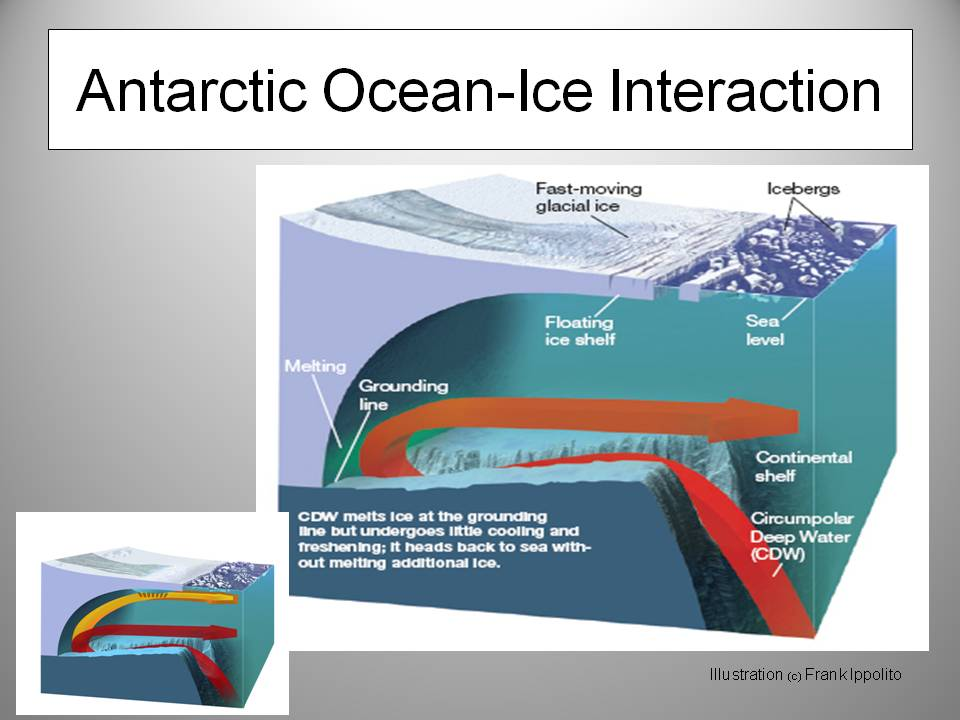
\includegraphics[width=\textwidth]{figures/GroundingLine/NaturalHistory2008} \\
  \vspace{-.5em}
  {\tiny Bindschadler 2008}
\end{frame}

\begin{frame}
  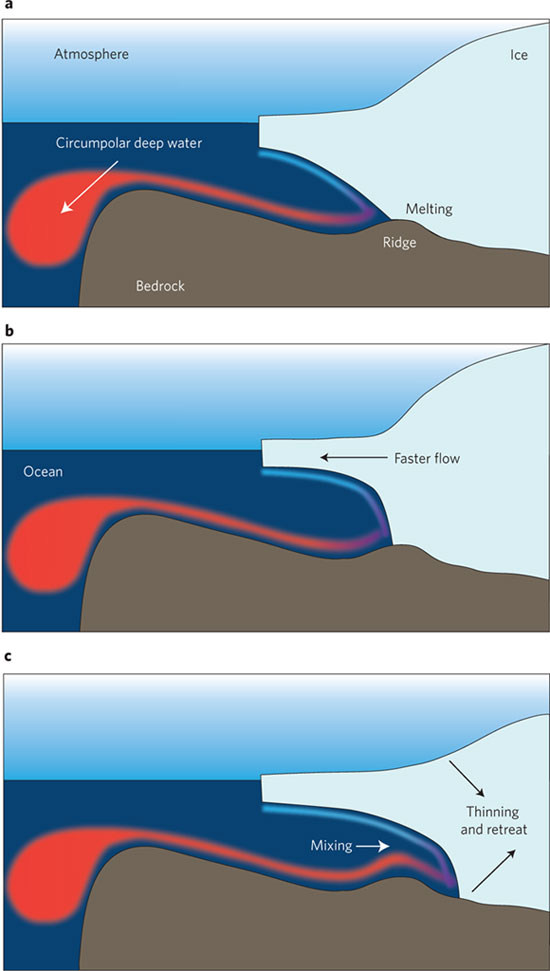
\includegraphics[width=0.5\textwidth]{figures/GroundingLine/SchoofNature2010}
\end{frame}

\begin{frame}{Grounding lines}
  \begin{columns}
    \begin{column}{0.45\textwidth}
      \centering
      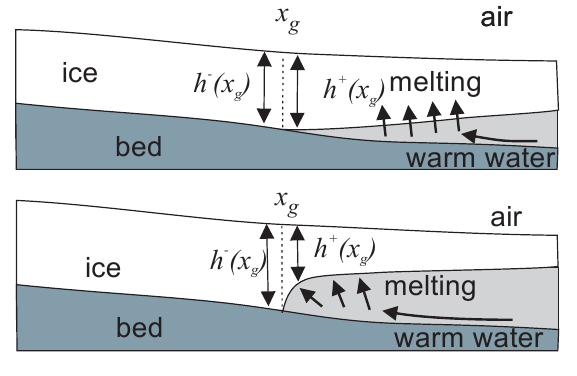
\includegraphics[width=\textwidth]{figures/GroundingLine/circulation} \\
      \vspace{-.5em}
      {\tiny Schoof 2007} \\
      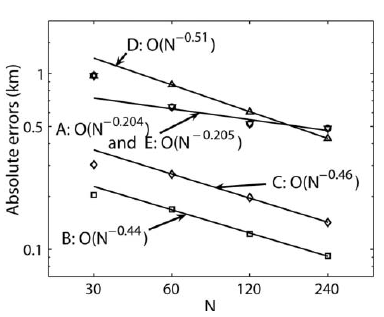
\includegraphics[width=\textwidth]{figures/GroundingLine/isothermal-Linfty} \\
      \vspace{-.5em}
      {\tiny Bueler et. al. 2005}
    \end{column}
    \begin{column}{0.55\textwidth}
      \begin{itemize}
      \item ocean circulation is very sensitive to grounding line
        geometry, feedback
      \item non-shallow physics applies in vicinity of grounding line
      \item current models are less than first-order accurate at margins
      \item extremely high resolution needed for qualitatively correct
        results on Eulerian meshes
      \end{itemize}
    \end{column}
  \end{columns}
\end{frame}

\begin{frame}{}
  \begin{columns}
    \begin{column}{0.63\textwidth}
      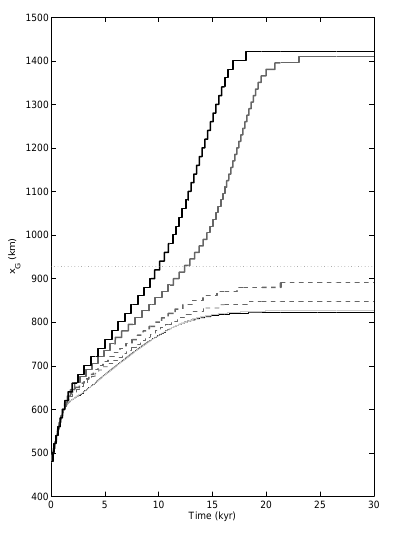
\includegraphics[width=\textwidth]{figures/GroundingLine/MeshDependence}
    \end{column}
    \begin{column}{0.35\textwidth}
      {\centering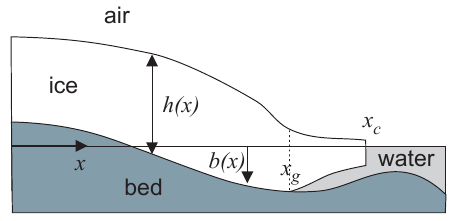
\includegraphics[width=1.2\textwidth]{figures/GroundingLine/SchoofGeom} \\
      \footnotesize{(Schoof 2007)}} \\
      \bigskip
      \bigskip
      Evolution of grounding line location on 20, 15, 10, 7.5 and 2.5 kilometer
        meshes in one horizontal dimension.  \footnotesize{(\emph{Durand et al. 2009})}
    \end{column}
  \end{columns}
\end{frame}

\begin{frame}{} %{Thwaites and Pine Island glaciers}
  \begin{columns}
    \begin{column}{0.1\textwidth} 
    \end{column}
    \begin{column}{.8\textwidth}
      \centering
      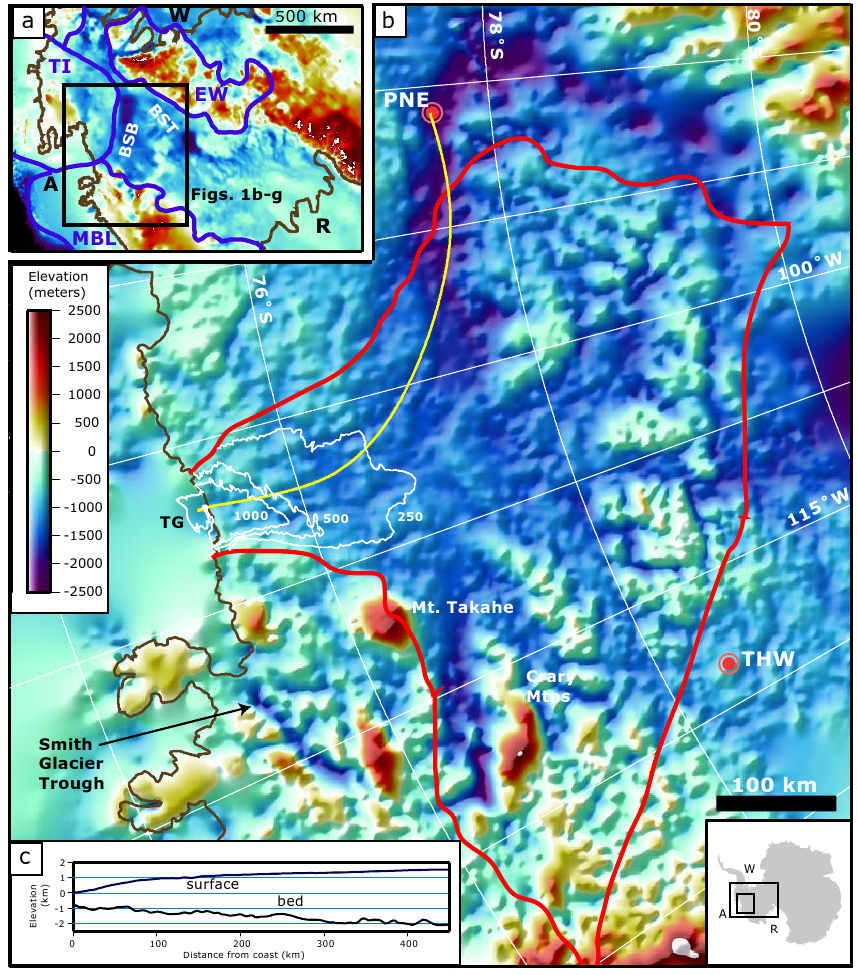
\includegraphics[width=0.95\textwidth]{figures/GroundingLine/thwaites}
    \end{column}
    \begin{column}{0.1\textwidth}
      {\tiny Holt \etal 2006}
    \end{column}
  \end{columns}
\end{frame}

\begin{frame}
  \begin{columns}
    \begin{column}{0.45\textwidth}
      \vspace{-1em}
      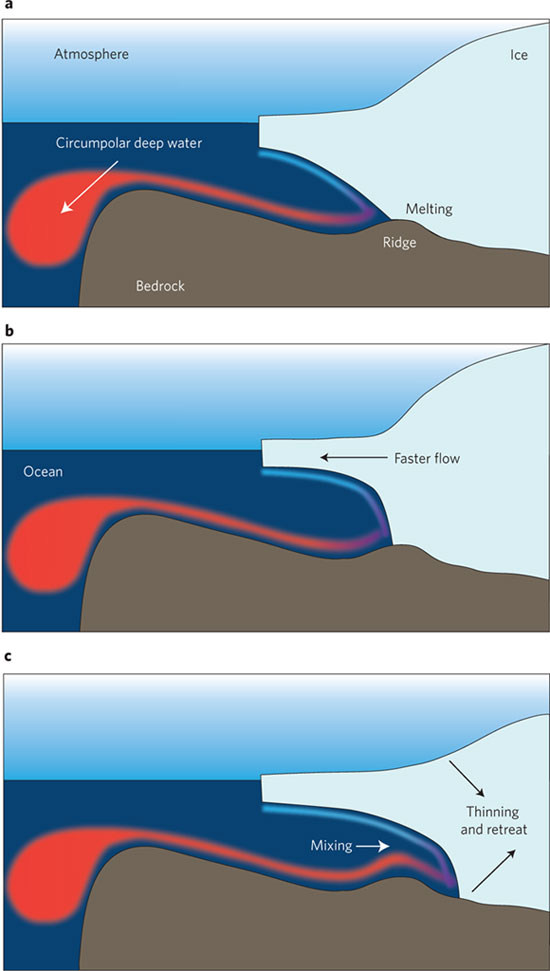
\includegraphics[width=\textwidth]{figures/GroundingLine/SchoofNature2010} \\
\footnotesize{(Schoof 2010)}
    \end{column}
    \begin{column}{0.55\textwidth}
      {\large \color{blue}{$y^+$ underneath an ice shelf}}
    \begin{itemize}
    \item Order of magnitude dimensions: length \unit{100}{\meter},       speed \unit{10}{\centi\meter\per\second}
    \item Viscous boundary layer: $y^+ \in \bigO(1) \implies       \unit{1}{\milli\meter}$ grid
    \item No-slip boundary conditions requires \emph{resolution} of this       layer % (wall resolution)
    \item Otherwise we need nonlinear slip
      \begin{itemize} \item still usually $y^+ \in \bigO(100)$       \end{itemize}
    \item Estimates come from validation (lab experiments) with heat       transfer in industrial and aerospace applications
    \item Thermohaline boundary layer: \unit{\text{1--10}}{\meter}
    \item Boundary layer equations require solution of a Riemann problem
    %\item Is simulation of this process plausible without boundary-fitted meshes?
    \end{itemize}
   \end{column}
  \end{columns}
\end{frame}

% \begin{frame}{$y^+$ underneath an ice shelf}
%   \begin{itemize}
%   \item Order of magnitude dimensions:
%     length \unit{100}{\meter}, speed \unit{10}{\centi\meter\per\second}
%   \item Viscous boundary layer: $y^+ \in \bigO(1) \implies % \unit{1}{\milli\meter}$ grid spacing
%   \item No-slip boundary conditions requires \emph{resolution} of this % layer % (wall resolution)
%   \item Otherwise we need nonlinear slip conditions
%     \begin{itemize} \item still usually $y^+ \in \bigO(100)$ % \end{itemize}
%   \item Estimates come from validation (lab experiments) with heat
%     transfer in industrial and aerospace applications
%   \item Thermohaline boundary layer is \unit{\text{1--10}}{\meter}
%   \item Boundary layer equations require solution of a Riemann problem
%   \item Is simulation of this process plausible without \\
%     boundary-fitted meshes?
%   \end{itemize}
% \end{frame}

\begin{frame}{LES+RANS with wall modeling}
  \begin{itemize}
  \item State of the art for high-Reynolds separating flows
  \item Subshelf circulation separates when it reaches neutral buoyancy \\ (this is a crucial limiting process)
  \item Is it possible to accurately predict heat transfer, separation, and overturning with $y^+ \in \bigO(10^5)$?
  \end{itemize}
  \begin{quotation}
    %Also, it
    It has been repeatedly observed, especially at high Reynolds     numbers and coarse grids and with the interface location being around     $y^+ = \bigO(100-200)$, that the high turbulent viscosity generated by     the turbulunce model in the inner region extends, as subgrid-scale     viscosity, deeply into the outer LES region, causing severe damping in     the resolved motion and a misrepresentation of the resolved structure as     well as the time-mean properties.
  \end{quotation}
  (Tessicini, Li, Leschziner, \emph{Simulation of Separation from Curved Surfaces with Combined LES and RANS Schemes}, 2007)
\end{frame}

\section{ALE Formulation}
\begin{frame}{Non-Newtonian Stokes system: velocity $\bm u$, pressure $p$}
\begin{columns}
\begin{column}{0.5\textwidth}
  \alert{\begin{align*}
    -\nabla \cdot(\eta D\uu) + \nabla p - \ff &= 0 \\
    \nabla \cdot \uu &= 0
  \end{align*}}
\end{column}
\begin{column}{0.5\textwidth}
    \begin{align*}
      D\uu &= \tfrac 1 2 \left(\nabla \uu + (\nabla \uu)^T \right) \\
      \gamma(D\uu) &= \tfrac 1 2 D\uu \tcolon D\uu \\
      \eta(\gamma) &= B(\Theta,\dotsc)\big(\epsilon + \gamma \big)^{\frac{\mathfrak{p}-2}{2}} \\
      \mathfrak{p} &= 1 + \tfrac{1}{\mathfrak{n}} \approx \tfrac 4 3 \\
      T &= \bm 1 - \bm n \otimes \bm n \\
    \end{align*}
\end{column}
\end{columns}
\vspace{-1.5em}
    with boundary conditions
    \begin{align*}
      (\eta D\bm u - p\bm 1)\cdot\bm n =
      \begin{cases}\bm 0 & \text{free surface} \\
        -\rho_w z \bm n & \text{ice-ocean interface}\end{cases} \\
      \bm u = \bm 0\qquad\qquad \text{frozen bed}, \Theta < \Theta_0 \\
      \left. \begin{aligned}
          \bm u \cdot \bm n &= \bm g_{\text{melt}}(T\uu,\dotsc) \\
          T (\eta D\bm u - p\bm 1)\cdot\bm n &= \bm g_{\text{slip}}(T \bm u,\dotsc) \end{aligned}\right\}
      \text{nonlinear slip}, \Theta \ge \Theta_0 \\
    \end{align*}
    \vspace{-3em}
    \[ \bm g_{\text{slip}}(T\uu) = \beta_{\mathfrak{m}}(\dotsc) \lvert T\bm u \rvert^{\mathfrak{m}-1} T \bm u \]
    Navier $\mathfrak{m}=1$, \quad Weertman $\mathfrak{m}\approx \frac 1 3$, \quad Coulomb $\mathfrak{m}=0$.
\end{frame}

\begin{frame}{Other critical equations}
  \vspace{-0.3em}
  \begin{itemize}
  \item Mesh motion: $\bm x$
    \begin{columns}
      \begin{column}{0.4\textwidth}
        \vspace{-1.5em}
        \begin{gather*}
          \alert{-\nabla\cdot\bm \sigma = 0} \\
          \text{surface: }(\bm {\dot{x}}- \bm u)\cdot\bm n = q_{BL},\;
          T\bm \sigma \cdot \bm n = 0
        \end{gather*}
      \end{column}
      \begin{column}{0.6\textwidth}
        \begin{gather*}
          \bm \sigma = \mu \Big[ 2 D\bm w + (\nabla \bm w)^T\nabla \bm w \Big] + \lambda|\nabla\bm w|\bm 1 \\
          \bm w = \bm x - \bm x_0 \\
        \end{gather*}
      \end{column}
    \end{columns}
\vspace{-1em}
  \item Heat transport: $\Theta$ (enthalpy)
    \begin{multline*}
      \frac{\partial}{\partial t} \Theta + {\color{blue} (\bm u - \bm{\dot{x}})}\cdot \nabla \Theta \\
      - \nabla\cdot \Big[ {\color{green!70!black} \kappa_T(\Theta)\nabla T(\Theta)} + {\color{magenta!70!black} \kappa_\omega\nabla \omega(\Theta) + \bm q_D(\Theta)} \Big] - {\color{cyan!70!black} \eta D\bm u\tcolon D\bm u} = 0
    \end{multline*}
    \vspace{-0.5em}
    \begin{itemize}
      \begin{columns}
        \begin{column}{0.2\textwidth}\end{column}
        \begin{column}{0.4\textwidth}
    \item {\color{blue} ALE advection}
    \item {\color{green!70!black} Thermal diffusion}
    \end{column}
    \begin{column}{0.4\textwidth}
    \item {\color{magenta!70!black} Moisture diffusion/Darcy flow}
    \item {\color{cyan!70!black} Strain heating}
    \end{column}
  \end{columns}
\end{itemize}
\vspace{0.3em}
    Note: $\kappa(\Theta)$ and $\bm q_D(\Theta)$ are very sensitive near $\Theta=\Theta_0$
\end{itemize}
\vspace{-.6em}
\begin{block}{Summary of primal variables in DAE}
  \begin{tabular}{lll}
    $u$ & velocity & algebraic \\
    $p$ & pressure & algebraic \\
    $x$ & mesh location & algebraic in domain, differential at surface \\
    $\Theta$ & enthalpy & differential
  \end{tabular}
\end{block}
\end{frame}

%\input{slides/Dohp/Resolution.tex}
\newcommand{\colorA}[1]{{\color{red} #1}}
\newcommand{\colorB}[1]{{\color{green!60!black} #1}}
\newcommand{\colorC}[1]{{\color{blue} #1}}
\newcommand{\colorD}[1]{{\color{magenta!70!black} #1}}
\newcommand{\colorE}[1]{{\color{cyan!70!black} #1}}
\newcommand{\colorF}[1]{{\color{yellow!60!black} #1}}
\newcommand{\colorG}[1]{{\color{red!50!white} #1}}

\begin{frame}{ALE form}
  After discretization in time ($\alpha \propto 1/\Delta t$) we have a Jacobian
  \begin{equation*}
    \begin{bmatrix}
      \colorA{A_{II}} & \colorA{A_{I\Gamma}}             &                       &                             &                     &   \\
      & \colorB{\alpha M_{\Gamma\Gamma}} &                       & \colorB{- N_{\Gamma\Gamma}} &                       &  \\
      \colorG{G_{II}}      & \colorG{G_{\Gamma I}} & \colorC{B_{II}}       & \colorC{B_{I\Gamma}}        & \colorC{C_{I}^T}    & \colorD{D_I} \\
      \colorG{G_{I\Gamma}} &        \colorG{G_{\Gamma\Gamma}}                          & \colorC{B_{\Gamma I}} & \colorC{B_{\Gamma\Gamma}}   & \colorC{C_{\Gamma}^T} & \colorD{D_\Gamma} \\
      \colorG{G_{Ip}}        &  \colorG{G_{\Gamma p}}                                & \colorC{C_{I}}        & \colorC{C_{\Gamma}}         &                   & \\
      \colorE{\alpha E_I}    & \colorE{\alpha E_\Gamma} & \colorE{F_I} & \colorE{F_\Gamma} & & \colorF{\alpha M_\Theta + J}
    \end{bmatrix}
    \begin{bmatrix}
      x_I \\ x_\Gamma \\ u_I \\ u_\Gamma \\ p \\ \Theta
    \end{bmatrix}
  \end{equation*}
  \begin{itemize}
  \item \colorA{mesh motion equations (Laplace-Beltrami or pseudo-elasticity)}
  \item \colorB{$(\dot{\bm x} - \bm u)\cdot \bm n = \text{accumulution}$}
  \item \colorG{``just'' geometry}
  \item \colorC{Stokes problem}
  \item \colorD{temperature dependence of rheology}
  \item \colorE{convective terms and strain heating in heat transport}
  \item \colorF{thermal advection-diffusion}
  \end{itemize}
\end{frame}

\begin{frame}{Power-law Stokes Scaling}
  \centering
  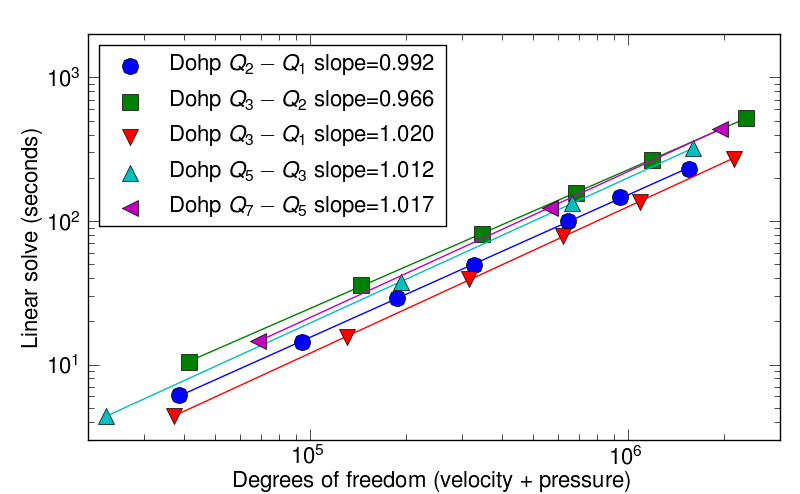
\includegraphics[width=\textwidth]{figures/Dohp/Stokes2} \\
  Only assemble $Q_1$ matrices, ML+PETSc smoothers for elliptic pieces \\
  (easy geometry and coefficients)
\end{frame}


\section{Conservation}
\begin{frame}{Artifacts of stabilization}
  \begin{columns}
    \begin{column}{0.4\textwidth}
      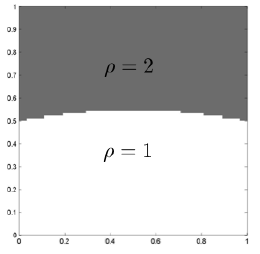
\includegraphics[width=\textwidth]{figures/Stabilization/RayleighTaylor} \\
      Rayleigh-Taylor initiation, isoviscous \\
      (Dave May and Yury Mishin)
    \end{column}
    \begin{column}{0.6\textwidth}
      $Q_2-P_{-1}$ (stable, locally conservative) \\
        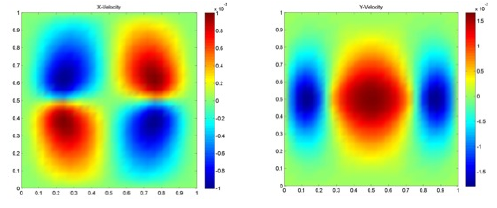
\includegraphics[width=\textwidth]{figures/Stabilization/Q2Pm1} \\
        \medskip
        $Q_1-Q_1$ (stabilized) \\
        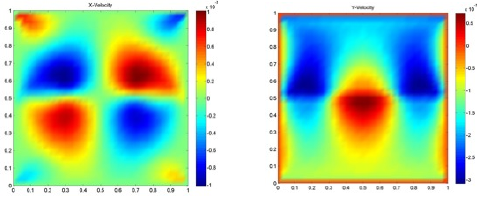
\includegraphics[width=\textwidth]{figures/Stabilization/Q1Q1stab} \\
        \vbox{\hspace{4em} $u$ \hspace{8em} $v$}
    \end{column}
  \end{columns}
\end{frame}


\section[Slip]{Slip boundary conditions on bumpy surfaces}
\begin{frame}{Construction of conservative nodal normals}
  \begin{gather*}
    \bm n^i = \int_\Gamma \phi^i \bm n
  \end{gather*}
  \begin{itemize}
  \item Exact conservation even with rough surfaces
  \item Definition is robust in 2D and for first-order elements in 3D
  \item $\int_\Gamma \phi^i = 0$ for corner basis function of undeformed $P_2$ triangle
  \item May be negative for sufficiently deformed quadrilaterals
  \item Mesh motion should use normals from CAD model
    \begin{itemize}
    \item Difference between CAD normal and conservative normal introduces correction term to conserve mass within the mesh
\item Anomolous velocities if disagreement is large \\ (fast moving mesh, rough surface)
    \end{itemize}
  \item Normal field not as smooth/accurate as desirable \\ (and achievable with non-conservative normals)
    \begin{itemize}
    \item Mostly problematic for surface tension
    \item Walkley et al, \emph{On calculation of normals in free-surface flow problems}, 2004
    \end{itemize}
  \end{itemize}
\end{frame}

\begin{frame}{Need for well-balancing}
  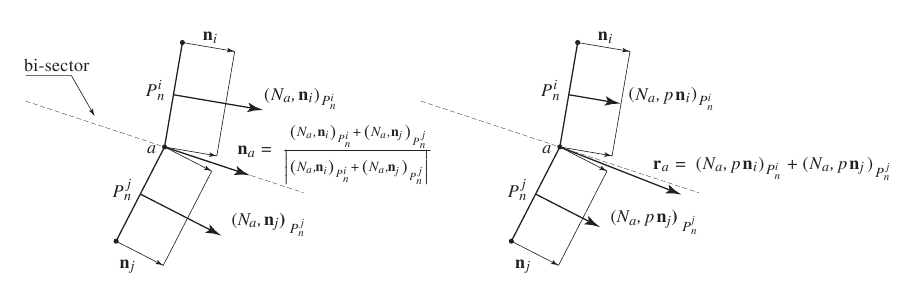
\includegraphics[width=\textwidth]{figures/slip/Behr2004-NormalVsResidual} \\
  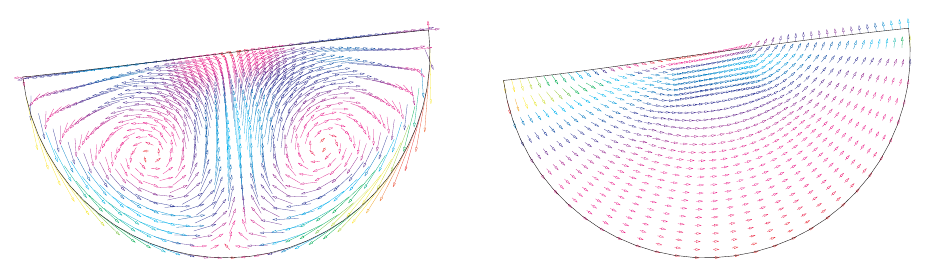
\includegraphics[width=\textwidth]{figures/slip/Behr2004-NavierSloshing} \\
  \footnotesize{(Behr, \emph{On the application of slip boundary condition on curved surfaces}, 2004)}
\end{frame}

\begin{frame}{``No'' boundary condition}
  \begin{itemize}
  \item Integration by parts produces
    \begin{gather*}
      \int_\Gamma \bm v \cdot T \bm\sigma \cdot \bm n, \qquad \bm\sigma = \eta D \bm u - p\bm 1, \qquad T = \bm 1 - \bm n \otimes \bm n
    \end{gather*}
  \item Continuous weak form requires either
    \begin{itemize}
    \item Dirichlet: $\bm u |_{\Gamma} = \bm f \implies \bm v|_\Gamma = 0$
    \item Neumann/Robin: $\bm\sigma\cdot\bm n |_\Gamma = \bm g(\bm u,p)$
    \end{itemize}
  \item Discrete problem allows integration of $\bm\sigma\cdot\bm n$ ``as is''
    \begin{itemize}
    \item Extends validity of equations to include $\Gamma$
    \item \alert{Not valid} for continuum equations
    \item Introduced by Papanastasiou, Malamataris, and Ellwood, 1992 for Navier-Stokes outflow boundaries
    \item Griffiths, {\small \emph{The `no boundary condition' outflow boundary condition}, 1997}
      \begin{itemize}
      \item Proves $L^\infty$ order of accuracy $\bigO((h + 1/\Peclet)^{p+1})$ \\
        for Galerkin finite elements of order $p$ (linear advection-diffusion)
      \item Demonstrates equivalence with collocation at Radau points \\ in outflow element
      \end{itemize}
    \item Used in slip boundary conditions by Behr 2004
    \end{itemize}
  \end{itemize}
\end{frame}


\section[Hydrostatic]{A robust multigrid solver for the hydrostatic equations}
\begin{frame}[shrink=5]{Hydrostatic equations for ice sheet flow}
  \begin{itemize}
  \item Valid when $w_x \ll u_z$, independent of basal friction {\small (Schoof\&Hindmarsh 2010)}
  \item Eliminate $p$ and $w$ from Stokes by incompressibility:\\
    \quad 3D elliptic system for $\bm u = (u,v)$
    \begin{align*}
      - \nabla\cdot \left[ \eta
        \begin{pmatrix}
          4 u_x + 2 v_y & u_y + v_x & u_z \\
          u_y + v_x & 2 u_x + 4 v_y & v_z
        \end{pmatrix} \right] + \rho g \bar\nabla h & = 0
    \end{align*}
    \begin{align*}
      \eta(\theta,\gamma) &= \frac{B(\theta)}{2} (\gamma_0 + \gamma)^{\frac{1-\mathfrak n}{2\mathfrak n}}, \qquad \mathfrak n \approx 3 \\
      \gamma &= u_x^2 + v_y^2 + u_xv_y + \frac 1 4 (u_y+v_x)^2 + \frac 1 4 u_z^2 + \frac 1 4 v_z^2
    \end{align*}
    and slip boundary $\sigma \cdot \bm n = \beta^2 \bm u$ where
    \begin{align*}
      \beta^2(\gamma_b) &= \beta_0^2 (\epsilon_b^2 + \gamma_b)^{\frac{\mathfrak m-1}{2}}, \qquad 0 < \mathfrak m \le 1 \\
      \gamma_b &= \frac 1 2 (u^2 + v^2)
    \end{align*}
  \item $Q_1$ FEM with Newton-Krylov-Multigrid solver in PETSc: \code{src/snes/examples/tutorials/ex48.c}
  \end{itemize}
\end{frame}

\frame{
  \vspace{-8em}
  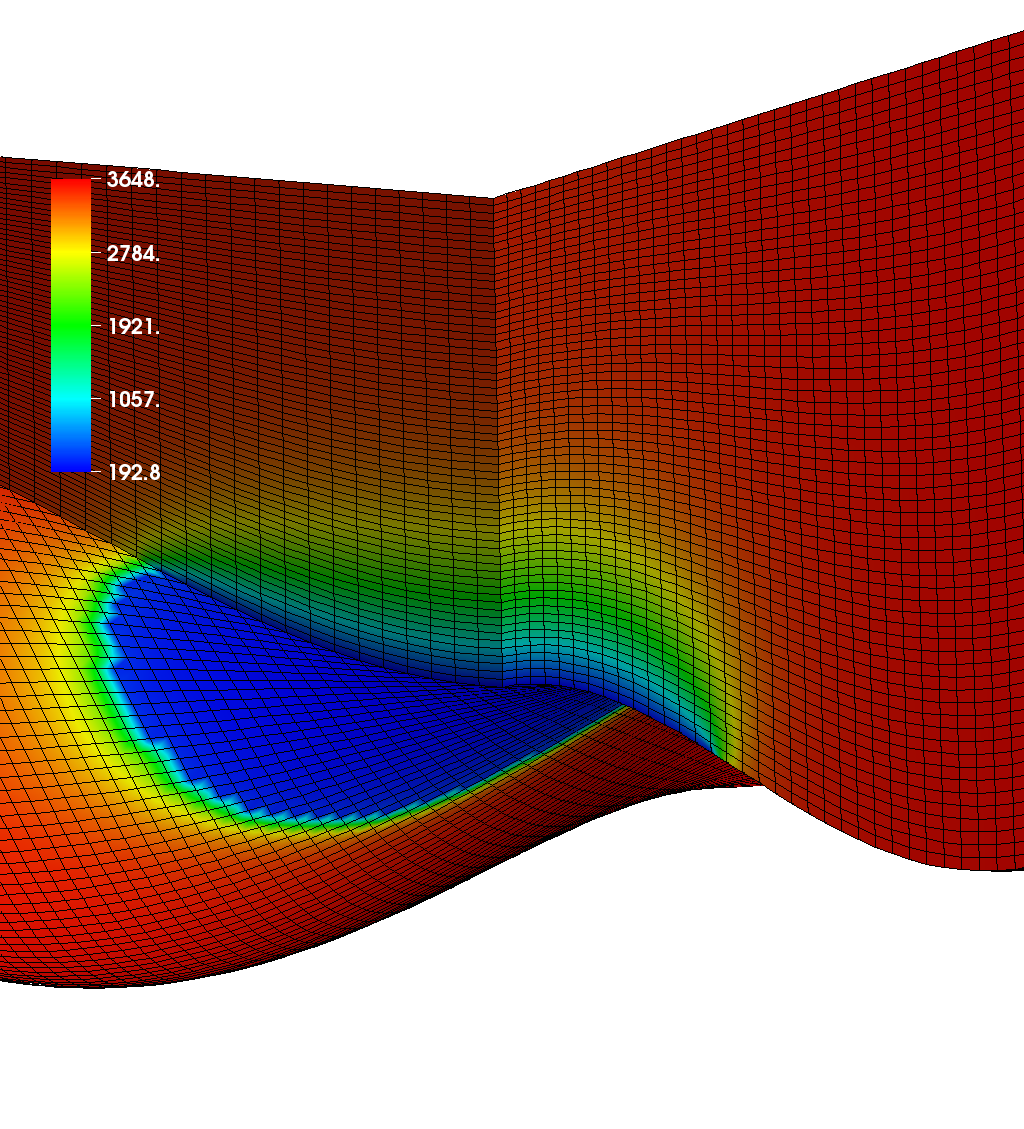
\includegraphics[width=1.2\textwidth]{figures/THI/x-5km-m8p5l5-clip}
}

\begin{frame}{What about splitting at the global level?}
  \begin{itemize}\footnotesize
  \item Split $(u,v)$ multiplicatively at global level: {\code{\small -pc\_type fieldsplit}}
    \begin{itemize} 
    \item parallel direct solve in splits \\
      {\code{-fieldsplit\_pc\_type cholesky -fieldsplit\_pc\_factor\_mat\_solver\_package mumps}}
    \item Split additively instead \\
      {\code{-pc\_fieldsplit\_type additive}}
    \item Parallel ML in splits, ASM(1)/ICC(1) on levels \\
      {\code{-fieldsplit\_pc\_type asm \\ \qquad -fieldsplit\_sub\_pc\_type icc \\ \qquad -fieldsplit\_sub\_pc\_factor\_levels 1}}
    \item Parallel BoomerAMG in splits \\
      {\code{-fieldsplit\_pc\_type hypre}}
    \item ASM/Cholesky in splits \\
      {\code{-fieldsplit\_pc\_type asm \\ \qquad -fieldsplit\_sub\_pc\_type cholesky}}
    \item ASM/ICC(0) in splits \\
      {\code{-fieldsplit\_pc\_type asm \\ \qquad -fieldsplit\_sub\_pc\_type icc}}
    \end{itemize}
  \end{itemize}
\end{frame}

\begin{frame}{Split in subdomains?}
  \begin{itemize}
  \item ASM on coupled system: {\code{-pc\_type asm}}
    \begin{itemize}
    \item Split in subdomains, Cholesky in splits \\
    {\code{-sub\_pc\_type fieldsplit \\ \qquad -sub\_fieldsplit\_pc\_type cholesky}}
    \item Split in subdomainst, ML in splits \\
      {\code{-sub\_pc\_type fieldsplit \\ \qquad -sub\_fieldsplit\_pc\_type ml}}
    \item Split in subdomains, BoomerAMG in splits \\
      {\code{-sub\_pc\_type fieldsplit \\ \qquad -sub\_fieldsplit\_pc\_type hypre}}
    \item Split in subdomains, ICC(1) in splits \\
      {\code{-sub\_pc\_type fieldsplit \\ \qquad -sub\_fieldsplit\_pc\_type icc}}
    \item Block ICC(0) on subdomains (no splitting), stored as block symmetric
      {\code{-sub\_pc\_type icc -da\_mat\_type sbaij}}
    \end{itemize}
  \end{itemize}
\end{frame}

\begin{frame}{Coupled Multigrids}
  \begin{itemize}
  \item Geometric multigrid with isotropic coarsening, ASM(1)/Cholesky and ASM(0)/ICC(0) on levels \\
    {\code{\small -mg\_levels\_pc\_type bjacobi -mg\_levels\_sub\_pc\_type icc -mg\_levels\_1\_pc\_type asm -mg\_levels\_1\_sub\_pc\_type cholesky}}
  \item \ldots with Galerkin coarse operators \\
    {\code{\small -pc\_mg\_galerkin}}
  \item \ldots with ML's aggregates \\
    {\code{\small -pc\_type ml -mg\_levels\_pc\_type asm}}
  \item Geometric multigrid with aggressive semi-coarsening, ASM(1)/Cholesky and ASM(0)/ICC(0) on levels \\
    {\code{\small -da\_refine\_hierarchy\_x 1,1,8,8 -da\_refine\_hierarchy\_y 2,2,1,1 -da\_refine\_hierarachy\_z 2,2,1,1}}
  \item Simulate 1024 cores, interactively, on my laptop \\
    {\code{\small -mg\_levels\_pc\_asm\_blocks 1024}}
  \end{itemize}
\end{frame}

\begin{frame}{Summary of solvers}
  \centering
  \begin{tabular}{|l|c|}
    \hline
    Method & Avg Krylov/Newton \\
    \hline
    Global multiplicative FieldSplit, ASM/LU & 175 \\
    Global multiplicative FieldSplit, BoomerAMG & 59 \\
    Global multiplicative FieldSplit, strong ML & 71 \\
    Global additive FieldSplit, ASM/LU & 197 \\
    Global ASM, FieldSplit/LU inside & 215 \\
    Global ASM, LU inside & 167 \\
    Coupled BoomerAMG & 60 \\
    Coupled ML with strong smoothers & 72 \\
    Geometric multigrid & 11 \\
    Geometric multigrid, Galerkin coarse & 122 \\
    \hline
  \end{tabular} \\
  {Smallish size $40\times 40\times 10$, relatively extreme parameters}
\end{frame}

\begin{frame}{Linear solve performance}
  \centering
  \includegraphics[width=\textwidth]{figures/THI/linear4}
\end{frame}

\begin{frame}{Status-quo Picard}
  \includegraphics[width=\textwidth]{figures/THI/z-picard-mult-noseq}
\end{frame}

\begin{frame}{Grid sequencing: \code{-dmmg\_grid\_sequence}}
    \includegraphics[width=0.9\textwidth]{figures/THI/z-mult-o1-r2}
\end{frame}

\begin{frame}{Avoid oversolving}
    \includegraphics[width=0.9\textwidth]{figures/THI/z-mult-o1-ew} \\
    Luis Chacon's variant of Eisenstat-Walker: \\
    \code{\footnotesize -snes\_ksp\_ew -snes\_ksp\_ew\_rtolmax 0.5 -snes\_ksp\_ew\_version 3}
\end{frame}


\begin{frame}{Outlook}
  \begin{block}{}
    \begin{itemize}
    \item Exact local conservation is critical for problems with discontinuous geometry and coefficients
    \item Nonlinear slip on irregular surfaces is hard but tractable (mostly)
    \item Smooth manufactured solutions are necessary, but not sufficient to study solver and discretization performance
    \item Need good software to combine relaxation for loosely coupled processes and factorization
      for stiff/indefinite coupling
    \item Modeling of boundary layer processes in highly anisotropic geometry likely requires conforming to the interface
    \end{itemize}    
  \end{block}
  \begin{block}{Tools}
    \begin{itemize}
    \item PETSc\ \url{http://mcs.anl.gov/petsc}
      \begin{itemize}\item ML, Hypre, MUMPS
      \end{itemize}
    \item ITAPS \url{http://itaps.org}
      \begin{itemize}\item MOAB, CGM, Lasso
      \end{itemize}
    \end{itemize}
  \end{block}
\end{frame}
\end{document}
